
%% This is file `elsarticle-template-1-num.tex',
%%
%% Copyright 2009 Elsevier Ltd
%%
%% This file is part of the 'Elsarticle Bundle'.
%% ---------------------------------------------
%%
%% It may be distributed under the conditions of the LaTeX Project Public
%% License, either version 1.2 of this license or (at your option) any
%% later version.  The latest version of this license is in
%%    http://www.latex-project.org/lppl.txt
%% and version 1.2 or later is part of all distributions of LaTeX
%% version 1999/12/01 or later.
%%
%% The list of all files belonging to the 'Elsarticle Bundle' is
%% given in the file `manifest.txt'.
%%
%% Template article for Elsevier's document class `elsarticle'
%% with numbered style bibliographic references
%%
%% $Id: elsarticle-template-1-num.tex 149 2009-10-08 05:01:15Z rishi $
%% $URL: http://lenova.river-valley.com/svn/elsbst/trunk/elsarticle-template-1-num.tex $
%%
\documentclass[preprint,12pt]{elsarticle}

%% Use the option review to obtain double line spacing
%% \documentclass[preprint,review,12pt]{elsarticle}

%% Use the options 1p,twocolumn; 3p; 3p,twocolumn; 5p; or 5p,twocolumn
%% for a journal layout:
%% \documentclass[final,1p,times]{elsarticle}
%% \documentclass[final,1p,times,twocolumn]{elsarticle}
%% \documentclass[final,3p,times]{elsarticle}
%% \documentclass[final,3p,times,twocolumn]{elsarticle}
%% \documentclass[final,5p,times]{elsarticle}
%% \documentclass[final,5p,times,twocolumn]{elsarticle}

%% if you use PostScript figures in your article
%% use the graphics package for simple commands
%% \usepackage{graphics}
%% or use the graphicx package for more complicated commands
%% \usepackage{graphicx}
%% or use the epsfig package if you prefer to use the old commands
%% \usepackage{epsfig}

%% The amssymb package provides various useful mathematical symbols
\usepackage{amssymb}
%% The amsthm package provides extended theorem environments
%% \usepackage{amsthm}

%% The lineno packages adds line numbers. Start line numbering with
%% \begin{linenumbers}, end it with \end{linenumbers}. Or switch it on
%% for the whole article with \linenumbers after \end{frontmatter}.
\usepackage{lineno}

%% natbib.sty is loaded by default. However, natbib options can be
%% provided with \biboptions{...} command. Following options are
%% valid:

%%   round  -  round parentheses are used (default)
%%   square -  square brackets are used   [option]
%%   curly  -  curly braces are used      {option}
%%   angle  -  angle brackets are used    <option>
%%   semicolon  -  multiple citations separated by semi-colon
%%   colon  - same as semicolon, an earlier confusion
%%   comma  -  separated by comma
%%   numbers-  selects numerical citations
%%   super  -  numerical citations as superscripts
%%   sort   -  sorts multiple citations according to order in ref. list
%%   sort&compress   -  like sort, but also compresses numerical citations
%%   compress - compresses without sorting
%%
%% \biboptions{comma,round}

% \biboptions{}


\usepackage[italian]{babel}

\usepackage[utf8]{inputenc}
\usepackage[T1]{fontenc}

\usepackage{listings}
\lstloadlanguages{C++}

\renewcommand{\lstlistingname}{Codice}

\usepackage{graphicx}

\usepackage{verbatim}

\journal{Journal Name}

\begin{document}

\begin{frontmatter}

%% Title, authors and addresses

%% use the tnoteref command within \title for footnotes;
%% use the tnotetext command for the associated footnote;
%% use the fnref command within \author or \address for footnotes;
%% use the fntext command for the associated footnote;
%% use the corref command within \author for corresponding author footnotes;
%% use the cortext command for the associated footnote;
%% use the ead command for the email address,
%% and the form \ead[url] for the home page:
%%
%% \title{Title\tnoteref{label1}}
%% \tnotetext[label1]{}
%% \author{Name\corref{cor1}\fnref{label2}}
%% \ead{email address}
%% \ead[url]{home page}
%% \fntext[label2]{}
%% \cortext[cor1]{}
%% \address{Address\fnref{label3}}
%% \fntext[label3]{}

\title{Corso di Metodi e Modelli per l'Ottimizzazione Combinatoria - Relazione progetto}


\address{Universit\'a degli studi di Padova \\ Anno Accademico 2015/2016}

%% use optional labels to link authors explicitly to addresses:
%% \author[label1,label2]{<author name>}
%% \address[label1]{<address>}
%% \address[label2]{<address>}

\author{\textbf{Studente:} Giacomo Quadrio \\\textbf{Matricola:} 1061566}
\end{frontmatter}

%%\begin{abstract}

\textbf{\abstractname{}}

%% Text of abstract
Il progetto del corso di Metodi e Modelli per l'Ottimizzazione Combinatoria consiste nel risolvere un problema che vede coinvolta un'azienda metalmeccanica che produce pannelli forati per la costruzione di quadri elettrici. La foratura di questi è eseguita attraverso un macchinario a controllo numerico dotato di una punta diamantata che, muovendosi sul pannello secondo una sequenza programmata, produce i fori nelle posizioni desiderate. L'obiettivo è quindi quello di individuare la sequenza di foratura ottimale che minimizzi i tempi di produzione, tenendo conto che il tempo necessario per la foratura è lo stesso e costante per tutti i punti. Il cosiddetto Problema del Commesso Viaggiatore, più comunemente noto come TSP (\textit{Travelling Salesman Problem}), in cui è richiesto di trovare il \textit{circuito Hamiltoniano} di costo complessivo minimo dato un grafo G = (V,E) pesato con costi c\begin{tiny}ij
\end{tiny} assegnati ad ogni arco (i,j). Un circuito Hamiltoniano non è altro che un ciclo all'interno del grafo tale che ogni vertice v $\in$ V appartenga al ciclo e venga percorso una sola volta. 

Nei problemi di tipo TSP abbiamo poi che i costi degli archi rispettano la cosiddetta \textit{disuguaglianza triangolare} ovvero dati tre punti A, B e C, la distanza tra A e C deve essere al massimo la distanza tra A e B più la distanza tra B e C. Più nel dettaglio il TSP in esame in questo progetto è un \textit{TSP euclideo} o planare cioè nel quale si usano le ordinarie distanze euclidee per i costi degli archi. Nonostante il problema rimanga NP-difficile molte euristiche riescono a lavorare meglio. 

%%
%% Start line numbering here if you want
%%
%%\linenumbers

%% main text
\section{Modello del problema}
\label{S:1}
Il problema oggetto del progetto pu\'o essere formulato come un problema di ottimizzazione su reti di flusso partendo quindi da un grafo G = (N,A). Scegliendo arbitrariamente un nodo di partenza 0 $\in$ N impostiamo ad $\mid$N$\mid$ il flusso uscente da esso in modo tale che venga spinto verso altri nodi. Tale operazione ha per\'o dei vincoli ovvero ciascun nodo, eccetto l'origine, ricever\'a una e una sola unit\'a di flusso, ogni nodo sia visitato una e una sola volta e che il costo del cammino, in termini di pesi c{\tiny ij}, sia minimo.

\subsection{\textbf{Il modello nella Programmazione Lineare Intera}}

Il problema può essere formalizzato con il seguente modello di programmazione lineare intera. Avremo quindi:
\\

\begin{large}
\textbf{Insiemi}
\end{large}

\begin{itemize}
\item \textbf{N:} nodi del grafo, rappresentano le posizioni dei fori da realizzare
\item \textbf{A:} insieme degli archi (i,j) con i e j $\in$ N. Essi rappresentano il tragitto per spostarsi dal nodo i al nodo j\\

\end{itemize}

\begin{large}
\textbf{Parametri}
\end{large}

\begin{itemize}
\item \textbf{c{\tiny ij}:} tempo impiegato per spostarsi dal nodo i al nodo j con i e j $\in$ N e l'arco (i,j) $\in$ A.
\item \textbf{0:} nodo di partenza del cammino $\in$ N.\\

\end{itemize}


\begin{large}
\textbf{Variabili decisionali}
\end{large}

\begin{itemize}
\item \textbf{x{\tiny ij}:} unità di flusso trasportate da i a j con i e j  $\in$ N e l'arco (i,j) $\in$ A.
\item \textbf{y{\tiny ij}:} indica l'utilizzo dell'arco (i,j), 1 se viene utilizzato, 0 altrimenti. Avremo che i e j  $\in$ N e l'arco (i,j) $\in$ A.\\

\end{itemize}

\begin{large}
\textbf{Vincoli\\}
\end{large}

Il modello, a questo punto, prevede un totale di cinque vincoli differenti che possono essere indicati come segue:


\begin{enumerate}
\item Il flusso uscente da x{\tiny 0j} deve essere massimo, cioè $\mid$N$\mid$
\item Ogni nodo utilizza al massimo una unità di flusso, tranne il nodo di partenza
\item Ogni nodo ha un solo arco in entrata
\item Ogni nodo ha un solo arco in uscita
\item Se vi è un'unità di flusso trasportata da i a j deve di conseguenza esserci un arco che va da i a j
\end{enumerate}

\section{Metaeuristiche scelte per il modello e loro implementazione}
\label{S:2}

Il progetto da svolgere richiesto dal corso di Metodi e Modelli per l'Ottimizzazione Combinatoria prevede la risoluzione del modello di programmazione lineare intera tramite due tecniche ovvero usando il risolutore IBM CPLEX ed una o più metaeuristiche a nostra scelta. Una volta fatto ciò si procederà testando i metodi con delle istanze di prova ed i risultati e statistiche confrontati tra di loro per valutarne le prestazioni.

Nello specifico, il problema in esame è un problema di ricerca di vicinato e consiste nel definire una soluzione iniziale e cercare di migliorarla esplorando un intorno di questa soluzione; quindi i metodi scelti ed utilizzati all'interno del progetto sono due, la Local Search ed il Simulated Annealing. Si tratta di metodi metaeuristici ovvero tecniche generali di schemi algoritmici concepiti indipendentemente dal problema specifico.Tali metodi definiscono delle componenti e le loro iterazioni al fine di pervenire ad una buona soluzione ed esse inoltre devono essere specializzate per i singoli problemi. \\

\subsection{\textbf{Descrizione delle metaeuristiche}}


\textbf{Local Search}: si definisce una soluzione iniziale e si cerca di migliorarla esplorando un intorno di questa soluzione. Se l'ottimizzazione sull'intorno della soluzione corrente produce una soluzione migliorante il procedimento viene ripetuto partendo, come soluzione corrente, dalla soluzione appena determinata. L'algoritmo termina quando non è più possibile trovare delle soluzioni miglioranti nell'intorno della soluzione corrente o quando è stata determinata una soluzione con valore della funzione obiettivo uguale a qualche bound.\\

\textbf{Simulated Annealing}: il concetto su cui si basa questa metodologia prende spunto dal mondo reale ovvero consiste nel simulare il comportamento di un processo termodinamico di ricottura di materiali solidi. Se un materiale solido viene riscaldato oltre il proprio punto di fusione e poi viene raffreddato in modo da riportarlo allo stato solido, le sue proprietà strutturali dipenderanno fortemente dal processo di raffreddamento. In sostanza tale algoritmo simula il cambiamento di energia di un sistema sottoposto a raffreddamento, fino a che non converge ad uno stato solido; ciò permette di cercare soluzioni ammissibili di problemi di ottimizzazione cercando di convergere verso soluzioni ottime. \\

\subsection{\textbf{Implementazione degli algoritmi}\\}

\begin{large}
\textbf{Risolutore IBM CPLEX}
\end{large}


Il risolutore IBM CPLEX è un programma di ottimizzazione che prende il nome dal metodo del simplesso implementato in linguaggio C (anche se ad oggi offre interfacce verso altri linguaggi ed ambienti). Esso trova soluzioni a problemi di programmazione lineare intera anche di notevoli dimensioni, utilizzando le varianti primale o duale del metodo del simplesso. L'implementazione eseguita per il progetto ricalca a grandi linee quanto fatto durante le lezioni di laboratorio: innanzitutto viene letta la matrice delle adiacenze e linearizzata in un array di dimensioni pari a n*n. Dopodiché si inseriranno in coda i costi degli archi c{\tiny ij} come coefficienti delle variabili decisionali y{\tiny ij}. A questo punto dovranno infine essere creati i vari vincoli definiti nel paragrafo 1.1, sotto la voce "Vincoli", attraverso appositi vettori. \\



\begin{large}
\textbf{Local Search}
\end{large}

\begin{lstlisting}[basicstyle=\small, caption={Local Search}, frame=single, language=C++]

sol = getInitialSol(random);

while (true){
	vector<int> newSol = findBestN(sol);
	if (evaluate(newSol) >= evaluate(sol)){	
		return evaluate(sol);
	}else{					
		sol = newSol;
	}
}


\end{lstlisting}


Come si può vedere, l'algoritmo di Local Search crea innanzitutto una soluzione iniziale da cui partire tramite la funzione getInitialSol, dopodiché esso è stato implementato utilizzando un unico ciclo while che opera finché non viene restituito in output un valore. Questo significa che ciò avverrà unicamente quando, dopo aver calcolato una nuova soluzione con newSol = findBestN(sol), il suo valore sarà peggiore del valore della soluzione corrente. Se così non è la soluzione corrente viene aggiornata alla soluzione appena calcolata ed il ciclo continua ad operare fino al punto in cui viene trovata una soluzione peggiorativa. \\

\begin{large}
\textbf{Simulated Annealing}
\end{large}


\begin{lstlisting}[basicstyle=\small, caption={Simulated Annealing}, frame=single, language=C++]

sol = getInitialSol(random);
n_passi = 100000.0 * n / 5;

while (step < n_passi){
	newSol = getNeigh(sol,2,true);			
	float de = evaluate(sol) - evaluate(newSol);
	if (de > 0){
		sol = newSol;
	}else{ 
		temp = 1-(step/n_passi);	
		double prob = exp((de)/temp);	
		srand(time(NULL)+for_random);		
		for_random = for_random + 1;
		
		if (prob*100 > (rand()%100) ){
			sol = newSol;
		}
	}
step ++; 
}

return(LocalSearch(sol));
	
\end{lstlisting}

Per quanto concerne invece l'algoritmo di Simulated Annealing, anch'esso crea innanzitutto una soluzione iniziale da cui partire tramite la funzione getInitialSol, dopodiché troviamo un ciclo while principale che opererà finché step <= n\_
passi; da notare che il numero di passi inoltre è dinamico così che cresca al crescere del numero di nodi coinvolti nel problema. In cosa consiste quindi questo algoritmo? Viene calcolata una nuova soluzione attraverso la funzione getNeigh, dopodiché verrà calcolata la differenza tra il valore della soluzione corrente e quello della nuova soluzione. Se il delta ottenuto è maggiore di zero significa che la nuova soluzione è migliorativa e quindi aggiornerò di conseguenza sol, se invece così non è procederemo in maniera differente rispetto alla Local Search. Andremo infatti a calcolare per prima cosa la temperatura di raffreddamento, valore che è coinvolto nel calcolo della probabilità di accettare una mossa peggiorativa. Questa probabilità è calcolata come segue:

\begin{center}
prob = exp( $\delta$/t)
\end{center}

dove $\delta$ è l'entità del peggioramento de e t è la temperatura temp di raffreddamento. Nel caso la probabilità prob sia maggiore di un numero random calcolato attraverso la funzione srand ciò comporterà appunto l'accettare la mossa peggiorativa, altrimenti essa verrà scartata. Come si modifica però la probabilità p? Essa diminuisce al crescere del peggioramento indotto dalla mossa stessa e cresce al crescere della temperatura t di processo.

Al termine delle operazioni eseguite tramite il ciclo while andremo ad effettuare infine una \textbf{fase di intensificazione} tramite l'operazione di Local Search eseguita sulla soluzione migliore calcolata in precedenza. Il motivo di ciò è che la Local Search è una tecnica relativamente economica in quanto a tempi di esecuzione e permette di raffinare ulteriormente la soluzione trovata.


\section{Descrizione dei test effettuati}
\label{S:3}

Per verificare le prestazioni degli algoritmi utilizzati nel progetto sono stati condotti diversi test con un numero ben definito di istanze per differenti tipologie di dataset. Nel dettaglio sono stati utilizzati quattro diversi dataset in cui i punti sono disposti come segue:

\begin{itemize}
\item \textbf{Distribuzione uniforme} ovvero uniformemente disposti all'interno dello spazio
\item In \textbf{cluster} e disposti in tre raggruppamenti
\item In \textbf{circoli} e disposti in tre circonferenze
\item In \textbf{linea} e disposti in tre linee \\
\end{itemize}


\begin{figure}[htbp]
\centering
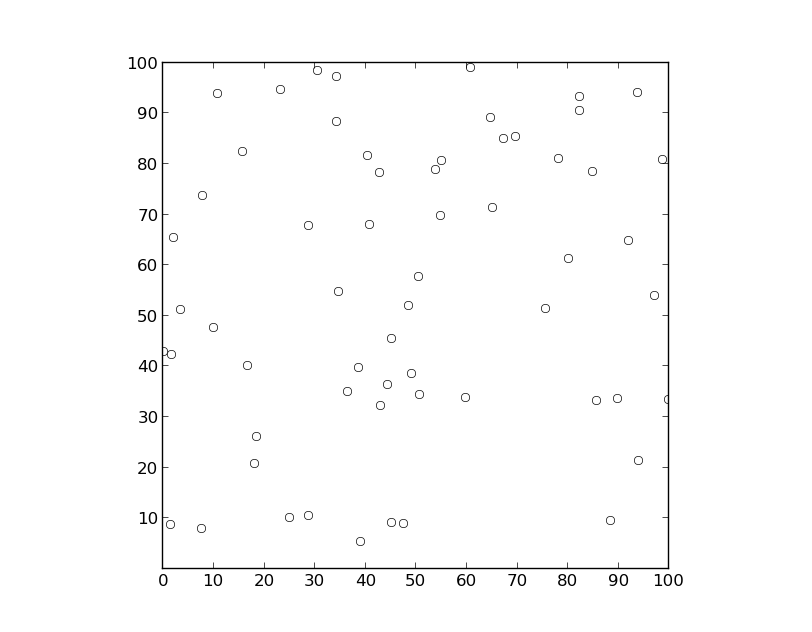
\includegraphics[scale=0.50]{grafici_istanze/random_60.png} 
\caption{Distribuzione uniforme}\label{fig:1}
\end{figure}

\begin{figure}[htbp]
\centering
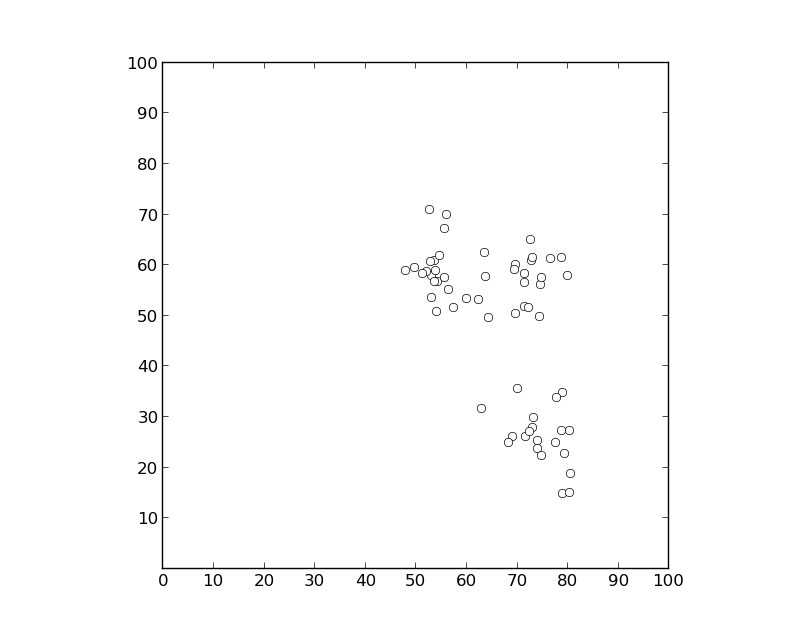
\includegraphics[scale=0.50]{grafici_istanze/cluster_60.png} 
\caption{Distribuzione in cluster}\label{fig:2}
\end{figure}

\begin{figure}[htbp]
\centering
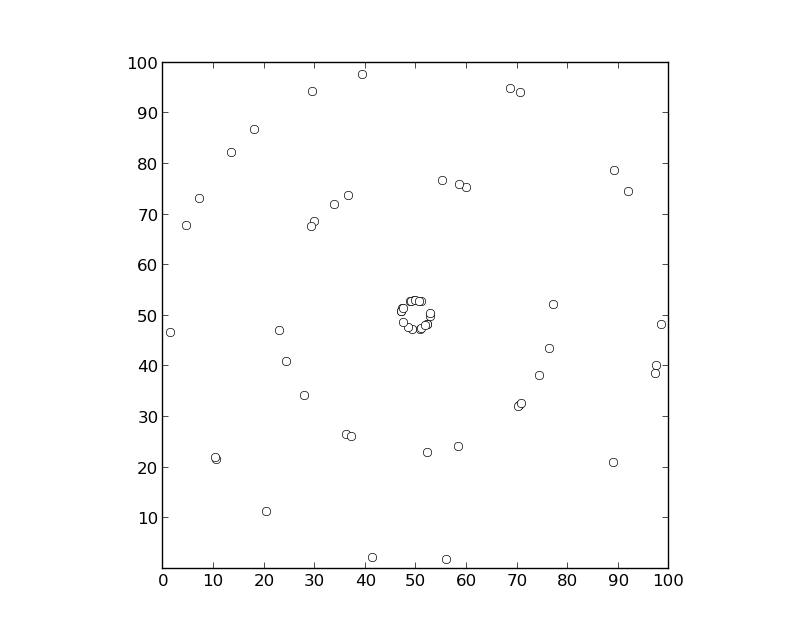
\includegraphics[scale=0.50]{grafici_istanze/circle_60.png} 
\caption{Distribuzione in cerchi}\label{fig:3}
\end{figure}

\begin{figure}[htbp]
\centering
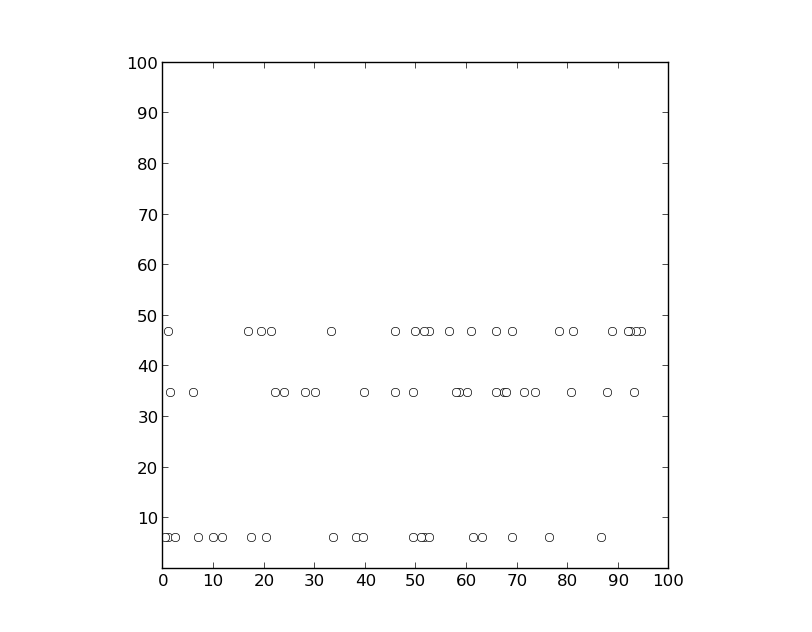
\includegraphics[scale=0.50]{grafici_istanze/line_60.png} 
\caption{Distribuzione in linee}\label{fig:4}
\end{figure}

Per ciascuna tipologia di dataset sono stati poi selezionati 10 raggruppamenti composti da 4 istanze, ognuno con un numero di nodi che va da 10 a 100 ed in cui la differenza della quantità di elementi tra un gruppo ed il successivo è pari a 10. Le istanze utilizzate sono in realtà matrici delle adiacenze M di dimensioni n*n tali che nella cella m\begin{tiny}ij\end{tiny} vi è la distanza tra il vertice v\begin{tiny}i\end{tiny} ed il vertice v\begin{tiny}j\end{tiny}

I test condotti per i vari algoritmi sono stati effettuati utilizzando, di volta in volta, sempre gli stessi dataset così da poter confrontare meglio i risultati. Ogni istanza di ogni raggruppamento di ogni dataset è stata infine data in pasto agli algoritmi per un totale di 10 volte ed i risultati registrati ritenuti interessanti per la valutazione sono stati vari quali il tempo medio e totale impiegato, il valore dell'ottimo, le soluzioni migliori, la varianza e via dicendo.

\begin{comment} %% Inizia il commento all'elenco puntato

\textbf{{\large Esecuzione utilizzando CPLEX:}
}\begin{itemize}
\item Tempo medio impiegato per le 10 esecuzioni di ogni istanza
\item Valore dell'ottimo\\
\end{itemize}

\textbf{{\large Esecuzione utilizzando la Local Search}
}\begin{itemize}
\item Tempo medio impiegato per le 10 esecuzioni di ogni istanza
\item Tempo totale impiegato dalle 10 esecuzioni
\item Miglior soluzione ottenuta con la sola Local Search
\item Peggior soluzione ottenuta con la sola Local Search
\item Media delle soluzioni ottenute con la sola Local Search
\item Varianza ottenuna
\end{itemize}

\textbf{
{\large Esecuzione utilizzando il Simulated Annealing:}}
\begin{itemize}
\item Tempo medio impiegato per le 10 esecuzioni di ogni istanza
\item Tempo totale impiegato dalle 10 esecuzioni
\item Miglior soluzione ottenuta con il Simulated Annealing
\item Peggior soluzione ottenuta con il Simulated Annealing
\item Media delle soluzioni ottenute con il Simulated Annealing
\item Varianza ottenuna
\item Miglior soluzione ottenuta con l'esecuzione della Local Search sui risultati del Simulated Annealing
\item Peggior soluzione ottenuta con l'esecuzione della Local Search sui risultati del Simulated Annealing
\item Media delle soluzioni ottenute con l'esecuzione della Local Search sui risultati del Simulated Annealing
\item Varianza ottenuna\\

\end{itemize}

\end{comment} %% Finisce il commento all'elenco puntato

\section{Descrizione dei risultati ottenuti}
\label{S:4}

I risultati completi ottenuti dall'esecuzione degli algoritmi sono stati riportati all'interno dei file Excel denominati "cplex\_results", "local\_search\_results", "sim\_annealing\_results" e non quindi direttamente nella relazione a causa della mole di dati che comprendono. In questa sede compariranno quindi solo risultati riassuntivi utili a meglio comprendere le conclusioni a cui si è giunti o, eventualmente, rimandi ai file sopraccitati. 

%% The Appendices part is started with the command \appendix;
%% appendix sections are then done as normal sections
%% \appendix

%% \section{}
%% \label{}

%% References
%%
%% Following citation commands can be used in the body text:
%% Usage of \cite is as follows:
%%   \cite{key}          ==>>  [#]
%%   \cite[chap. 2]{key} ==>>  [#, chap. 2]
%%   \citet{key}         ==>>  Author [#]

%% References with bibTeX database:

\bibliographystyle{model1-num-names}
\bibliography{sample.bib}

%% Authors are advised to submit their bibtex database files. They are
%% requested to list a bibtex style file in the manuscript if they do
%% not want to use model1-num-names.bst.

%% References without bibTeX database:

% \begin{thebibliography}{00}

%% \bibitem must have the following form:
%%   \bibitem{key}...
%%

% \bibitem{}

% \end{thebibliography}


\end{document}

%%
%% End of file `elsarticle-template-1-num.tex'.
